% Journal of Computational Science submission draft.
% CAS single-column template supplied by the author (2026-10-26).
% Verify the author roles and add the public data/code archive before submission.
\documentclass[a4paper,fleqn]{cas-sc}

\usepackage[numbers,sort&compress]{natbib}
\usepackage{amsmath,amssymb,booktabs,graphicx,siunitx}

\newcommand{\RelLTwo}{\mathrm{RelL2}}
\newcommand{\PDE}{\mathrm{PDE}}
\newcommand{\curv}{\mathrm{curv}}
\newcommand{\grad}{\mathrm{grad}}

\begin{document}
\let\WriteBookmarks\relax
\def\floatpagepagefraction{1}
\def\textpagefraction{.001}

\shorttitle{Physics penalties versus smoothness}
\shortauthors{X. Yan}
\title[mode=title]{Do physics-informed losses add value beyond smoothness? Controlled comparisons for neural PDE surrogates}

\author[1]{Xiaochen Yan}[orcid=0009-0002-9280-4323]
\cormark[1]
\ead{xiaochen-yan@qq.com}
\credit{Conceptualization, Data curation, Formal analysis, Investigation, Methodology, Software, Validation, Visualization, Writing -- original draft, Writing -- review and editing}
\affiliation[1]{organization={Independent Researcher},
  city={Shenzhen}, state={Guangdong}, country={China}}
\cortext[1]{Corresponding author}

\begin{abstract}
Physics-informed losses can improve neural PDE surrogates through generic regularization as well as equation-specific information. We compare resolved-band PDE residual penalties with matched gradient and curvature penalties using a fixed Fourier neural operator (FNO), paired budgets, and training-only calibration. On a locked 500-trajectory holdout from PDEBench one-dimensional Burgers, all penalties reduce mean per-trajectory relative $L^2$ error versus data-only training. The PDE gain is 1.38\%, with no established advantage over gradient smoothing; curvature smoothing is better by 0.00344 in absolute relative-$L^2$ error (registered trajectory-bootstrap interval [0.002879, 0.004032] for PDE minus curvature). Secondary Burgers comparisons do not establish a consistent PDE advantage over the strongest smoothness control. On synthetic periodic Allen--Cahn, a uniform interval constraint and a matched time-pointwise, spatially projected PDE penalty have virtually identical mean field errors both on development cases and on 200 new trajectories evaluated with the same 24 frozen fits. Fresh-set interval-minus-pointwise differences are $+4.52\times10^{-7}$ (dense) and $-8.15\times10^{-6}$ (sparse), less than 0.008\% of the pointwise means. These trajectory-bootstrap intervals condition on three fitted seeds and do not establish equivalence or replicate training. Field gains coexist with initial-time and derivative-error trade-offs. The tested PDE penalties can regularize predictions, but do not establish a general benefit beyond matched smoothness penalties.
\end{abstract}

\begin{highlights}
\item Matched smoothness controls explain much of the measured PDE-loss benefit.
\item Curvature smoothing outperforms the resolved PDE penalty on a locked Burgers holdout.
\item Fresh Allen--Cahn trajectories preserve the near-equal interval and pointwise means.
\item Sparse-label gains coexist with initial-time and derivative-error trade-offs.
\item 200 new Allen--Cahn cases evaluate frozen models in the same distribution.
\end{highlights}

\begin{keywords}
scientific machine learning \sep neural PDE surrogate \sep Fourier neural operator
\sep physics-informed learning \sep smoothness regularization \sep PDEBench
\end{keywords}

\maketitle

\section{Introduction}
Neural operators approximate maps between function spaces and are increasingly used as surrogates for repeated PDE solves, with DeepONet and Fourier neural operators as established formulations \citep{lu2021deeponet,kovachki2023neuraloperator,li2021fno,karniadakis2021sciML}. Physics-informed training adds a differential residual to data-fitting objectives, as in physics-informed neural networks and physics-informed neural operators \citep{raissi2019pinn,li2021pino}. Integral and variational residual formulations are also established approaches \citep{kharazmi2021vpinn}. These methods can improve predictions when labels are sparse or noisy, but a reduction in prediction error relative to an unregularized model does not by itself show that the governing equation supplied information beyond an ordinary smoothness prior.

This distinction matters in computational PDE learning. Differential residuals act on spatial and temporal derivatives, and their numerical evaluation depends on resolution, boundary representation, spectral truncation, and the learned solution's regularity. A derivative penalty can therefore improve a field metric even when it does not uniquely encode the relevant dynamics. A useful comparison must retain the same architecture and data, include derivative-based controls, and report field and structural errors together.

Prior analyses also document failure modes associated with ill-conditioned PDE residual objectives and imbalanced gradients among composite loss terms \citep{krishnapriyan2021characterizing,wang2021understanding}. These findings motivate treating matched smoothness penalties as substantive comparators rather than relying only on an unregularized baseline.

We present a controlled diagnostic study of PDE penalties against matched smoothness penalties. The main Burgers experiment uses a fixed FNO and a held-out set locked before its labels were opened. Secondary Burgers stress studies vary temporal supervision, label noise, spatial subsampling, and training-set size. A separate periodic Allen--Cahn study compares a joint interval constraint with a time-pointwise PDE constraint under dense and sparse temporal labels. After freezing all 24 fitted models, we evaluated them on 200 new trajectories from the same declared initial-condition distribution; this tests case generalization, not independent retraining.

Our contribution is empirical and bounded:
\begin{enumerate}
  \item We compare a resolved-band Burgers residual with matched gradient and curvature penalties under a locked architecture and training protocol, retaining a trajectory-level holdout for the registered comparison.
  \item We report negative and mixed outcomes under sparse-time, noisy-label, sample-count, and resolution conditions instead of selecting only favorable regimes.
  \item We compare same-architecture pointwise and interval Allen--Cahn constraints, then evaluate the frozen fits on new trajectories; the interval form has no practically material advantage over the pointwise form.
\end{enumerate}

We do not introduce a new network, residual, regularizer, or numerical identity. We do not claim that physics losses are generally equivalent to smoothing, that PINNs are ineffective, or that an integral constraint is superior to pointwise physics.

\section{Experimental design}
\subsection{Evidence tiers and datasets}
The study combines three evidence tiers, summarized in Table~\ref{tab:design}. The principal confirmatory comparison is the Burgers holdout locked before evaluation. Burgers stress tests and Allen--Cahn results are secondary evidence. All reported IDs have been consumed within this project; none is presented as an available future holdout.

\begin{table}
\centering\small
\caption{Study components and evidence status. Scores from distinct rows use different tasks, time windows, and metrics and must not be compared across rows.}
\label{tab:design}
\setlength{\tabcolsep}{3pt}
\begin{tabular}{p{0.18\linewidth}p{0.26\linewidth}p{0.25\linewidth}p{0.23\linewidth}}
\toprule
Component & Task and data & Main comparison & Evidence status \\
\midrule
Burgers primary & PDEBench 1D Burgers, $\epsilon=0.001$, 100 training trajectories; 256-point inputs; five supervised times & no penalty, resolved PDE, gradient, curvature & 500 trajectories selected after model/rule lock; now consumed \\
Burgers stress & Same public source; sparse times, 10\% noisy future labels, 128-point grid, or 20/50/100 training trajectories & no penalty, PDE, gradient, curvature & Reused project split; exploratory summaries \\
Allen--Cahn interval & Synthetic periodic Allen--Cahn; 100 training and 200 development trajectories; dense or endpoint-only time labels & no penalty, full curvature, interval, pointwise PDE & Development pool plus 200 new trajectories for inference-only confirmation of 24 frozen fits \\
\bottomrule
\end{tabular}
\end{table}

The Burgers data come from the public PDEBench release \citep{takamoto2022pdebench}. The source HDF5 file has 10,000 trajectories, 201 solution times, and 1,024 cell-centered spatial values per time; its SHA-256 is recorded in the supplementary reproducibility record. We use the dataset's $\nu=0.001$ file, but the upstream generator uses diffusion coefficient $\epsilon/\pi$; the residual uses $0.001/\pi$ rather than silently identifying the filename parameter with the equation coefficient. Spatial samples are taken at stride four for the primary 256-point setting, without an anti-alias filter.

The Allen--Cahn trajectories are synthetic, generated by the project's spectral solver for the classical reaction--diffusion equation \citep{allen1979}:
\begin{equation}
  u_t = 0.01 u_{xx} + 5u(1-u^2), \qquad x\in[-1,1) \text{ periodic}, \quad t\in[0,0.5].
  \label{eq:allen}
\end{equation}
The field is represented on 256 spatial points and generated from 12-mode random Fourier initial conditions. The original pool 200000--200299 was reused for model development; a later deterministic repartition uses 100 training and 200 development cases, with 68 development cases appearing in an earlier training split. A separate set 320000--320199 was generated only after model weights were frozen and was used for inference-only confirmation. These new trajectories are independent cases from the same synthetic distribution, not an independent model-training replication or a second PDE.

\subsection{Fixed FNO and data protocol}
All physics-versus-smoothness comparisons keep the FNO architecture fixed within each experiment. The continuous-time Burgers model has four spectral blocks, width 16, 16 retained modes, and 34,209 real parameters. It maps the initial field and query coordinates $(t,x)$ to a field prediction. The Burgers primary protocol uses 100 training trajectories and five time labels $t\in\{0,0.1,0.25,0.5,1\}$; training begins with 1,500 data-only updates followed by 750 paired continuation updates. Three training seeds are used. The final checkpoint is evaluated; there is no validation-selected checkpoint or seed.

For the Allen--Cahn study, the same parameter count and four-block FNO are used with a single periodic scalar coordinate feature. This feature changes positional information but does not hard-enforce periodicity. The model has a zero-initialized final output head. Dense supervision uses $t\in\{0,0.05,0.125,0.25,0.5\}$; sparse supervision uses only $t\in\{0,0.5\}$. Each condition has three seeds, a 1,500-step warm fit, and paired 750-step continuations. Sparse training statistics and loss calibration use only the two observed training labels. The complete cache contains five fields and is read for integrity checks, so we do not claim that unobserved field bytes were never loaded.

\subsection{Losses and calibration}
Let $u_\theta(t,x)$ denote the FNO prediction and $\mathcal{P}_{16}$ projection onto Fourier modes 0--16. The Burgers residual is
\begin{equation}
  r_B = \mathcal{P}_{16}\left[u_t + u u_x - \frac{0.001}{\pi}u_{xx}\right].
  \label{eq:burgers-residual}
\end{equation}
The matched smoothness controls penalize $\|\mathcal{P}_{16}u_x\|_2^2$ and $\|\mathcal{P}_{16}u_{xx}\|_2^2$. The same resolved band is used for the PDE, gradient, and curvature terms in the Burgers regularization study. The total objective is a normalized data loss plus a calibrated penalty. Penalty multipliers are set on training-only probes to a fixed initial penalty-to-data gradient-norm ratio; validation data choose among the prespecified multiplier values. The three-value grid is not an exhaustive tuning of either family, and selected settings lie at a grid boundary in the main comparison.

The Allen--Cahn pointwise constraint is a time-JVP residual evaluated at the same five quadrature nodes used by the interval condition and spatially projected to modes 0--16. For nodes $t_j=c+h\{-1,-1/2,0,1/2,1\}_j$, Simpson weights $\alpha=(1,4,2,4,1)/12$, and $F(u)=0.01u_{xx}+5u(1-u^2)$, define
\begin{align}
  \mathcal{L}_{\mathrm{point}} &= \mathbb{E}\!\left[\sum_j \alpha_j \left\|\mathcal{P}_{16}\left(u_t(t_j)-F(u(t_j))\right)\right\|_2^2\right], \\
  \mathcal{L}_{\mathrm{interval}} &= \mathbb{E}\!\left[\left\|\mathcal{P}_{16}\left(\frac{u(c+h)-u(c-h)}{2h}-\sum_j\alpha_jF(u(t_j))\right)\right\|_2^2\right].
  \label{eq:allen-losses}
\end{align}
The interval loss uses $h\in\{0.005,0.01\}$ and the same five-node query layout. Both losses use the observed-training target scale and an initial gradient ratio of 0.3. The pointwise objective is a time-pointwise, spatially projected PDE penalty; it is not a full-space, unrestricted PINN residual. The two loss formulations are not claimed to be statistically equivalent.

\subsection{Metrics and comparisons}
The primary field metric is mean per-trajectory relative $L^2$ error,
\begin{equation}
  \RelLTwo = \frac{1}{N}\sum_{i=1}^{N}\frac{\|u_i-\widehat u_i\|_2}{\|u_i\|_2}.
  \label{eq:rel-l2}
\end{equation}
For multi-time experiments, the metric is averaged over the time points registered for that condition. Relative first- and second-spatial-derivative errors are secondary structural metrics, computed on the native output grid with spectral derivatives and a fixed denominator floor derived from clean training data. The initial-condition score is reported separately and is not included in future-time means.

For the primary Burgers holdout, five pairwise contrasts were specified before target extraction: each penalty versus no penalty, PDE versus gradient, and PDE versus curvature. We use 10,000 paired trajectory bootstrap replicates with Bonferroni adjustment; the resulting intervals are conditional on the three fitted model seeds and do not quantify training-seed uncertainty. The minimum effect marker was 1\%. For the Allen--Cahn development comparison, no equivalence margin or confirmatory test was set. The later fresh-trajectory comparison uses two registered contrasts and reports Bonferroni-adjusted 97.5\% paired intervals, conditional on the same three frozen fits; no equivalence margin or training-seed inference is claimed.

\subsection{Software and AI-assisted research support}
The experiments, synthetic reference trajectories, and metric calculations were produced by the documented Python and spectral-solver programs. OpenAI Codex assisted with development and debugging of parts of the data-preparation, training/evaluation, audit, and plotting code, and with manuscript restructuring and drafting. Numerical outputs were computed by the recorded programs from the specified data and protocols rather than generated directly by a language model. The author is responsible for reviewing the software, provenance, results, references, and final manuscript.

\section{Results}
\subsection{A locked Burgers holdout shows regularization gains, not a unique PDE advantage}
All three penalties improve on the data-only model in the locked 500-trajectory Burgers holdout (Table~\ref{tab:burgers-confirm}). The PDE penalty lowers mean relative $L^2$ error by 1.376\%, while gradient and curvature penalties lower it by 1.439\% and 2.561\%, respectively. The PDE-minus-gradient interval includes zero. The PDE-minus-curvature contrast is positive throughout its adjusted interval, indicating that the tested curvature penalty has lower field error in this fixed setup. These intervals are trajectory-level and conditional on the three trained seeds.

\begin{table}
\centering\small
\caption{Primary Burgers holdout (500 trajectories). Lower error is better. Gains are relative to the data-only mean.}
\label{tab:burgers-confirm}
\begin{tabular}{lrr}
\toprule
Training objective & Mean per-trajectory relative $L^2$ & Gain vs. data only \\
\midrule
Data only & 0.290253 & -- \\
Resolved PDE penalty & 0.286260 & 1.376\% \\
Resolved gradient penalty & 0.286076 & 1.439\% \\
Resolved curvature penalty & \textbf{0.282820} & 2.561\% \\
\midrule
PDE $-$ gradient & $+0.000184$ & adjusted interval $[-0.000086,\ 0.000440]$ \\
PDE $-$ curvature & $+0.003440$ & adjusted interval $[+0.002879,\ +0.004032]$ \\
\bottomrule
\end{tabular}
\end{table}

The selected multiplier for each family was determined on development data from a three-value grid, with the upper value selected in the primary comparison. The result therefore compares the locked selected candidates, not fully optimized PDE and smoothness families. This qualification narrows the inference: the data show that the tested PDE penalty helps over no penalty, but do not establish a general ranking over all possible smoothness controls. Figure~\ref{fig:relative-gains} summarizes the condition-specific field-error changes; the registered uncertainty estimates apply to the paired Burgers contrasts in Table~\ref{tab:burgers-confirm}.

\begin{figure}
\centering
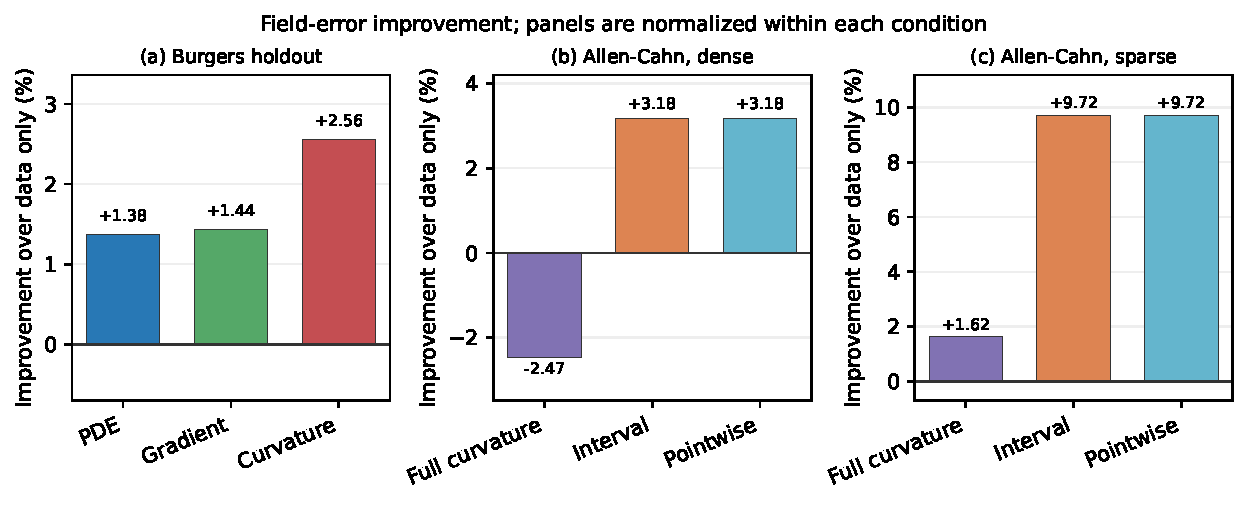
\includegraphics[width=0.88\linewidth]{figures/relative_gains.pdf}
\caption{Relative field-error improvement over the data-only baseline, computed separately within each evaluation condition. Positive values indicate lower error. The Burgers panel reports a locked 500-trajectory holdout; both Allen--Cahn panels report reused development data. No Allen--Cahn error bars are shown here because these bars summarize three fitted seeds on development cases. The separate fresh-trajectory contrast and its conditional bootstrap intervals are reported in Table~\ref{tab:allen-fresh}. The Burgers registered intervals apply to paired contrasts, not to individual bars.}
\label{fig:relative-gains}
\end{figure}

The registered mean contrasts conceal case-level variation. Figure~\ref{fig:paired-differences} displays the empirical distribution of paired, per-trajectory relative-$L^2$ differences on the 500-case Burgers holdout. Errors are first averaged across the three fitted seeds for each trajectory; negative values favor the PDE penalty. This is a descriptive view of the same consumed confirmation set, not an additional test or an independent estimate of training-seed uncertainty.

\begin{figure}
\centering
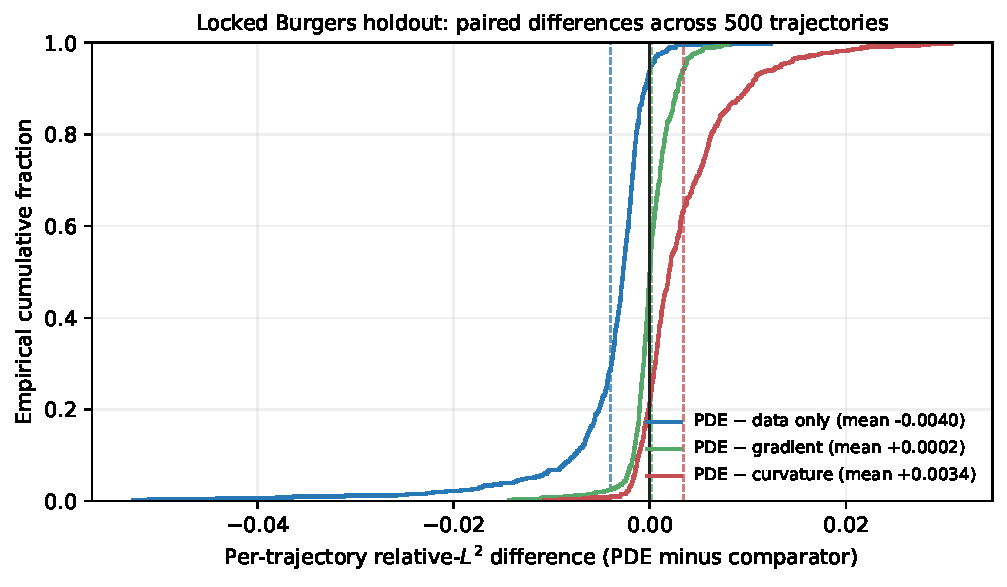
\includegraphics[width=0.78\linewidth]{figures/paired_burgers_differences.pdf}
\caption{Empirical cumulative distributions of paired per-trajectory relative-$L^2$ differences on the locked Burgers holdout. Each trajectory's error is averaged across the three model seeds before subtraction. Negative values favor the PDE penalty; positive values favor the comparator. Colored dashed vertical lines mark the corresponding mean differences. These descriptive distributions reuse the same 500 trajectories and do not replace the registered bootstrap intervals in Table~\ref{tab:burgers-confirm}.}
\label{fig:paired-differences}
\end{figure}

\subsection{Stress tests retain negative and mixed outcomes}
The Burgers stress experiments reuse project trajectories and are not independent confirmation. Under sparse time labels, 10\% noise on observed future labels, and their combination, PDE regularization reduces error relative to data-only fitting, but curvature smoothing has lower error in all three registered conditions (Table~\ref{tab:stress}). The noise is applied to training targets only; these results do not test noisy inputs. The synthetic Allen--Cahn pilot using the earlier linear-coordinate model gives a small 0.839\% field-error reduction for PDE versus no penalty, while curvature smoothing is worse than no penalty. This is a descriptive development result and is not pooled with the later periodic-coordinate Allen--Cahn experiments.

\begin{table}
\centering\small
\caption{Secondary fixed-architecture stress results. Entries are three-seed means of the condition-specific primary field metric. They use different task/time definitions and must only be read within each row.}
\label{tab:stress}
\begin{tabular}{lrrrr}
\toprule
Condition & Data only & PDE & Gradient & Curvature \\
\midrule
Burgers, sparse time labels & 0.644463 & 0.603849 & -- & 0.589233 \\
Burgers, 10\% noisy future labels & 0.273533 & 0.270520 & -- & 0.267287 \\
Burgers, sparse and noisy & 0.648667 & 0.611887 & -- & 0.599397 \\
\midrule
\multicolumn{5}{l}{Earlier synthetic Allen--Cahn pilot (linear coordinate; development only)} \\
Allen--Cahn, dense labels & 0.043007 & 0.042646 & -- & 0.043966 \\
\bottomrule
\end{tabular}
\end{table}

An additional Burgers sample-count and spatial-subsampling study reports three-seed means in Table~\ref{tab:sample-resolution}. At 256 and 128 points, the PDE and curvature means are nearly tied. At 20, 50, and 100 training trajectories, the PDE mean is higher than the better of the two displayed smoothness means. These rows reuse the project's original fixed-ID Burgers split and use a two-snapshot finite-difference residual rather than the continuous-time JVP residual of the primary study. We treat them as descriptive negatives only: the archived summary bootstraps three seed-level aggregates and also selects the better smoothness family from test outcomes, so those intervals do not support inferential claims.

\begin{table}
\centering\small
\caption{Descriptive Burgers resolution and sample-count results. Three-seed mean relative $L^2$ errors; no inferential interval is used.}
\label{tab:sample-resolution}
\begin{tabular}{lrrrr}
\toprule
Setting & Data only & PDE & Gradient & Curvature \\
\midrule
256 points, $n=1000$ & 0.208337 & 0.205374 & 0.216689 & 0.205024 \\
128 points, $n=1000$ & 0.208841 & 0.205445 & 0.216130 & 0.205399 \\
$n=20$, 256 points & 0.528445 & 0.513482 & 0.449342 & 0.479830 \\
$n=50$, 256 points & 0.4960 & 0.4166 & 0.3873 & 0.3781 \\
$n=100$, 256 points & 0.4230 & 0.3560 & 0.3517 & 0.3364 \\
\bottomrule
\end{tabular}
\end{table}

The two resolution rows are same-resolution training and evaluation at different spatial sampling rates; they are not cross-resolution generalization tests. The finite-difference time derivative spans stored indices 100 to 150 and is sensitive to the chosen temporal spacing. Neither study tests extrapolation to a new viscosity.

\subsection{Fresh Allen--Cahn trajectories preserve the interval--pointwise similarity}
Table~\ref{tab:allen} reports field and derivative errors for the development comparison on the reused Allen--Cahn pool. Under dense supervision, interval and pointwise field means differ by $4.5\times10^{-7}$ in absolute relative-$L^2$ error. Under sparse supervision, the interval mean is lower by $8.3\times10^{-6}$, but only two of three seed-level comparisons favor it. These development results do not establish formal equivalence or an interval advantage.

\begin{table}
\centering\scriptsize
\caption{Allen--Cahn development-set means over three model seeds. Lower values are better. Primary field windows differ between dense (four future times) and sparse (three omitted interior times), so dense and sparse magnitudes are not a direct treatment contrast.}
\label{tab:allen}
\begin{tabular}{llrrr}
\toprule
Labels & Continuation & Field relative $L^2$ & Gradient error & Curvature error \\
\midrule
Dense & Data only & 0.029808 & 0.110598 & 0.311226 \\
Dense & Full-frequency curvature & 0.030543 & 0.111206 & \textbf{0.290382} \\
Dense & Uniform interval & 0.028859 & 0.106258 & 0.297404 \\
Dense & Pointwise PDE nodes & \textbf{0.028859} & \textbf{0.106257} & 0.297402 \\
\midrule
Sparse & Data only & 0.128842 & 0.274621 & 0.675469 \\
Sparse & Full-frequency curvature & 0.126755 & \textbf{0.240080} & \textbf{0.534994} \\
Sparse & Uniform interval & \textbf{0.116313} & 0.248563 & 0.611276 \\
Sparse & Pointwise PDE nodes & 0.116321 & 0.248583 & 0.611329 \\
\bottomrule
\end{tabular}
\end{table}

Relative to data-only training, the interval and pointwise groups improve their condition-specific field means by approximately 3.18\% (dense) and 9.72\% (sparse). Both physical groups worsen mean initial-condition error by 2.26\% under dense labels and 6.76\% under sparse labels. The full-frequency curvature control has lower curvature error in the dense condition and lower gradient and curvature errors in the sparse condition, while its sparse field error is higher than the two PDE groups. No single objective dominates all metrics.

The development pool had already been used in earlier model and constraint development; the latest split contains 68 cases previously used for training. All 24 continuations and 18 historical control replays passed the registered artifact audit. This audit establishes artifact consistency, not independent scientific replication. The next check uses new trajectories but does not retrain the models.

After the 24 model fits were frozen, we generated 200 new initial conditions with IDs 320000--320199 and evaluated all 24 checkpoints without calibration or selection. Table~\ref{tab:allen-fresh} reports the paired interval-minus-pointwise differences. Dense supervision gives a difference of $+4.52\times10^{-7}$ (97.5\% trajectory-bootstrap interval [$3.43\times10^{-7}$, $5.59\times10^{-7}$]); sparse supervision gives $-8.15\times10^{-6}$ (interval [$-8.77\times10^{-6}$, $-7.55\times10^{-6}$]). The differences are $+0.00163\%$ and $-0.00712\%$ of the pointwise means. The intervals exclude zero, but they resample trajectories after averaging the same three fitted seeds and therefore do not measure training-seed variability. No equivalence margin was set. The result supports near-identical predictive means for these two losses on new cases; it does not support formal equivalence or a material interval advantage.

On these new cases, the interval and pointwise field means are descriptively 3.07\% lower than data-only under dense labels and about 9.3\% lower under sparse labels. The full-curvature control retains lower sparse gradient and curvature errors, and both physical fits retain higher initial-time error than data-only. These trade-offs remain consistent with the development analysis. The new cases confirm generalization of the frozen fits within the same initial-condition distribution; they do not provide an independent training replication, distribution-shift test, or second-PDE result.

\begin{table}
\centering\scriptsize
\caption{Fresh-trajectory Allen--Cahn confirmation. Difference is interval minus pointwise; intervals are 97.5\% paired trajectory-bootstrap percentile intervals, conditional on the three frozen fits.}
\label{tab:allen-fresh}
\begin{tabular}{lrrrr}
\toprule
Labels & Interval mean & Pointwise mean & Difference & 97.5\% interval \\
\midrule
Dense & 0.027689008 & 0.027688556 & $+4.52\times10^{-7}$ & [$3.43\times10^{-7}$, $5.59\times10^{-7}$] \\
Sparse & 0.114505896 & 0.114514050 & $-8.15\times10^{-6}$ & [$-8.77\times10^{-6}$, $-7.55\times10^{-6}$] \\
\bottomrule
\end{tabular}
\end{table}

\section{Discussion}
The main result separates two questions. First, does adding a penalty help relative to an unregularized fit? In the locked Burgers holdout, all three tested penalties do. Second, does the PDE residual improve prediction beyond a matched derivative penalty? In the same holdout, the answer is not established against gradient smoothing and is negative against the selected curvature penalty. The sparse/noisy Burgers stress outcomes show the same ordering descriptively. The results therefore do not support treating a gain over data-only fitting as evidence of equation-specific predictive information.

The interval comparison also narrows the interpretation of weak or integral consistency losses. On the fixed short windows studied here, a time-pointwise, low-frequency projected PDE objective yields practically the same means as the interval objective on both development and fresh trajectories. This is compatible with the two objectives being numerically close under the chosen nodes and warm predictions, but our training-probe algebraic diagnostic does not establish that closeness as a cause of the final field scores. The fresh-set bootstrap difference is conditional on three fitted seeds, and no equivalence margin was specified; this remains a bounded case-generalization observation, not a formal equivalence result.

The structural metrics expose trade-offs that a scalar field score would hide. In sparse Allen--Cahn supervision, the interval and pointwise terms have lower field error than the data-only and full-curvature means, but the full-curvature model retains substantially lower gradient and curvature errors. Each physical continuation also worsens the initial-condition score. These outcomes caution against describing a field-only improvement as a general increase in physical fidelity.

\subsection{Limitations}
The strongest confirmatory evidence covers one public PDE, one viscosity, one spatial sampling rate, and seen-time evaluation. Its model-selection grid is small and reaches its upper boundary, so the comparison is not an exhaustive search over regularization strengths or formulations. The bootstrap intervals quantify variation across held-out trajectories conditional on three fitted seeds, not uncertainty over training procedures. The secondary Burgers stress experiments reuse previously inspected data, and their confidence calculations are not used here because their effective resampling unit is only three seed-level summaries.

The Allen--Cahn experiments use synthetic trajectories and one reused development pool, plus a separate 200-trajectory set used to evaluate the same 24 frozen fits. Their pointwise physics term is spatially projected to modes 0--16 and uses time JVPs at five fixed nodes; it is not a full-space PINN comparison. The confirmation does not replicate training or test a shifted distribution. We also did not test noisy labels, cross-resolution transfer, long-time extrapolation, or a second unseen PDE. The periodic scalar coordinate does not itself enforce periodic boundary values or derivatives. We report these boundaries explicitly rather than extrapolating the observed rankings.

\section{Conclusion}
Under the tested fixed-architecture protocols, PDE penalties can improve neural PDE surrogate field error relative to data-only fitting, but the measured gains do not establish a general advantage over matched smoothness regularization. A locked Burgers holdout favors curvature smoothing over the selected PDE penalty, while the PDE-versus-gradient comparison remains unresolved. On Allen--Cahn, new trajectories preserve the near-identical interval and pointwise means of the development study for the frozen fits, alongside initial-time and derivative-error trade-offs. This is a trajectory-level confirmation within one synthetic distribution, not independent model retraining or second-PDE validation. The appropriate conclusion is conditional and diagnostic; no new architecture or universally superior physical loss is demonstrated.

\printcredits

\section*{Funding}
This research received no specific grant from any funding agency in the public, commercial, or not-for-profit sectors.

\section*{Declaration of competing interest}
The author declares no known competing financial interests or personal relationships that could have appeared to influence the work reported in this paper.

\section*{Data and code availability}
The PDEBench Burgers source data are available from the DaRUS PDEBench Datasets record (version 8.0; DOI: 10.18419/darus-2986)\citep{pdebench_dataset}; the source file used here is identified by the SHA-256 recorded in the supplementary material. The code, experiment protocols, split manifest, derived metrics, and synthetic Allen--Cahn materials, including the new trajectory evaluation set, are held in the author's private GitHub repository and are not publicly accessible at present. The raw PDEBench file and model/optimizer checkpoints are not included. All Allen--Cahn comparison cases reported here have been consumed; no future holdout is claimed.

\section*{Declaration of generative AI and AI-assisted technologies in the manuscript preparation process}
During the preparation of this work, the author used OpenAI Codex to assist with research-code development and debugging, data analysis and figure preparation, and manuscript restructuring and drafting. The author reviewed and edited the AI-assisted material as needed and takes full responsibility for the content of the article.

\footnotesize
\setlength{\bibsep}{0pt}
\bibliographystyle{elsarticle-num}
\bibliography{references}

\end{document}
